\documentclass[12pt,czech]{article}

\usepackage[utf8]{inputenc}
\usepackage[IL2]{fontenc}
\usepackage{helvet}
\usepackage[czech]{babel}
\usepackage[a4paper,textheight=674pt]{geometry}
\usepackage{xcolor}
\usepackage{hyperref}
\usepackage{graphicx}

% Default images path
\graphicspath{{project-plan/assets/}}

% Change default font family
\renewcommand{\sfdefault}{phv}
\renewcommand{\rmdefault}{phv}

% Visible todos
\newcommand{\todo}[1]{\noindent{\Large\color{red}TODO: #1}\par}

\title{Podnikatelský plán}
\author{Josef Doležal}

\begin{document}

\begin{titlepage}
    \vspace*{10cm}
	\centering
    
\includegraphics[width=4cm]{BI-EMP/project-plan/assets/logo}\par\vspace{1.5cm}
	{\LARGE What2Do \par}
	\vspace{1.5cm}
	{\huge\bfseries Podnikatelský plán\par}
	\vspace{1.5cm}
	{\Large\itshape Josef Doležal\par}
	\vfill

	{\large \today\par}
\end{titlepage}

\newpage
\tableofcontents

\newpage
\section{What2Do -- Marketingová geolokační platforma}

\vfill

\textbf{{\large Podnikatelský plán}}\smallskip\\*
Podnikatelským plánem společnosti What2Do je marketingová platforma, umožňující intereagovat s uživateli na základě jejich aktuální polohy a jejich volnočasových aktivit.
Díky unikátnímu využití moderních technologí umožňuje platforma velmi přesně určit cílovou skupinu nabízených služeb.

\vfill
\noindent What2Do, s.~r.~o.\\*
Karolinská 651\\*
186 00, Praha 8

\newpage
\section{Úvodní shrnutí}

\subsection{Podnikatelský záměr}

Cílem společnosti je vybudovat marketingovou platformu s využitím cílených nabídek na základě aktuální polohy koncového uživatele.
Platforma bude uživateli nabízet pouze relevantní služby v jeho okolí.
Tyto služby navíc budou zaměřené na impulzivní reakci uživatele.
Budou tedy časově omezené a nabízené pouze v danou chvíli.

\medskip

Kromě využití v marketingovém odvětví si společnost klade za cíl rozšířit platformu do geolokačních her a projektu chytrých měst.

\subsection{Faktory úspěchu}

Základním faktorem úspěchu vznikající platformy je její jedinečnost.
Přestože projekty s podobným konceptem již ve světě vznikly, jejich provedení nebylo technicky tak pokročilé, aby dokázalo zákazníky oslovit.

Pro získání strategických partnerů poskytujících obsah pro naši platformu chceme využít samotné uživatele, kteří jejich obsah budou vyžadovat.

\medskip

Důležitým krokem k úspěšnému navázání obchodních styku s komernčními partnery bude vytvoření poptávky po službách.
Té chceme dosáhnout tak, že uživatelům nabídneme obsah vybraných partnerů jako jsou divadla, muzea či jiné populárně kulturní organizace.

Na základě úspěchu v hlavním městě Praze se bude odvíjet následné rozšiřování platformy do dalších měst, případně států.

\subsection{Konkurenční výhoda}

Oproti konkurenci nabízíme našim klientům velmi úzce specifikovanou množinu uživatelů.
Běžné reklamy a jiné formy propagace navíc cílí na obecné požadavky uživatelů.
Přestože tím osloví větší uživateskou základnu, potýkají se s nízkým konverzním poměrem.

Naše platforma se navíc soustředí na opětovné oslovování stávajících uživatelů, nikoliv na akvizici potencionálních nových.

\subsection{Finanční náročnost a návratnost}

Z~počátku projektu bude finančně nejnáročnější pořízení geolokačních zařízení a~dostatečné počítačové infrastruktury pro zprovoznění webové části projektu.

Náklady na samotný provoz a rozšiřování geolokačních zařízení budou hrazené z~poplatků komerčních partnerů.

Návratnost projektu odhadujeme v průběhu druhého roku aktivního provozu v závislosti na počtu partnerů.

\newpage
\section{Společnost}

\subsection{Právní forma společnosti}

Jedná se o společnost s ručením o mezeným.
Zakládajícími členy jsou tři osoby, jejichž zaměření pokrývá potřebné znalosti pro vytvoření základní části projektu.
Spolumajitelé mají společnost rozdělenu rovným dílem.

Sídlo firmy se nachází v pražské čtvrti Karlín, kde společnost získala do pronájmu kancelářské prostory od jednoho ze strategických partnerů.
Kancelářské prostory jsou sdílené a výše nájmu se odvíjí od měsíčního využívání.

\subsection{Lokalita provozu}

Přestože kanceláře společnosti se nachází v pražském Karlíně, probíhat zde bude především softwarový vývoj.
Ostatní činnosti týkající se provozu společnosti a skladování potřebných materiálů se bude odehrávat ve skladových prostorech v Horních Počernicích.

Tyto prostory jsou majetkem společnosti.
Jejich využitím k provozním účelům se tak snižují náklady na kanceláře.

\subsection{Cíle}

Krátkodobé cíle společnosti se zaměřují na získání partnerů, jejichž služby mají neziskový charakter a jsou v současné době populární.
Společně s těmito partnery se pokusíme vybudovat stálou uživatelskou základnu.
Na základě popularity služby mezi touto skupinou uživatelů budeme službu rozšiřovat mezi komernční partnery, kteří jsou strategičtí pro finanční vyváženost projektu.

\medskip

Z dlouhodobého hlediska si klademe za cíl službu zpopularizovat mezi širokou veřejností.
Spolu s vysokou popularitou předpokládáme i nárůst počtu partnerů a s tím související zvyšující se výnosy.
Důraz bude kladen nejen na kvantitu poskytovaných služeb, ale především na kvalitu.

Dle našich uvážení je podstatné uživatelům poskytovat nejen placené služby, ale i služby spojené s jejich každodenními činnostmi.
Na základě této strategie se domníváme, že uživatelé si na poskytované služby navyknou a budou více naklokeni využívání služeb nových.

Touto formou se také budou odvíjet zejména marketingové aktivity naší společnosti.
Více o těchto aktivitách je uvedeno v části \ref{marketing}.

\newpage
\section{Popis podnikatelské příležitosti}

\subsection{Popis produktu}

Cílem společnosti je vytvořit úplně nový formát marketingových a reklamních sdělení prezentovaných pomocí mobilních zařízení.
Platforma, kterou budeme poskytovat umožňuje našim klientům a partnerům cílit na své uživatele v konkrétní čas a podle konkrétního místa.

Možnosti využití jsou téměř bezmezné.
Vzhledem k flexibilitě použitých technologií může mezi nabízené služby patřit běžné reklamní sdělení, časově omezené nabídky či nabídky unikátně vytvořené na míru pro specifické uživatele.

Platforma se ale neomezuje pouze na využití v marketingovém odvětví.
Pomocí našeho systému je možné vytvořit geoolokační hry, navigaci v budovách či umožnit prodej zboží.

\medskip

Prvními partnery jsou muzea, divadla a kina na území hl.~m.~Prahy.
Ty budou uživatele upozorňovat, pokud se v jejich okolí např. hraje v nadcházejících chvílích film, divadelní hra či kdy nejdříve jede z daného místa spoj městské hromadné dopravy.

\medskip

Platforma se tedy v počátku skládá z webového (administračního) rozhraní a knihoven pro systém iOS.
Administrační rozhraní i knihovny pro mobilní zařízení jsou vyvíjeny přímo ve společnosti.

\subsection{Užitek pro zákazníka}

Náš produkt si slibuje širokou uživatelskou základnu díky automatizování běžných činností.
Oproti běžnému formátu nabízení služeb vsázíme na strategii \textit{push-based}.
Tedy jediné co uživatel musí udělat, aby nabídku dostal, je pohybovat se ve specifických lokalitách.
Mobilní zařízení samo zjistí, že uživatel se vyskytl v okolí nabízené služby a službu mu nabídne.

V této fázi si slibujeme velkou konverzi uživatelů, protože cílíme na jejich impulzivní rozhodnutí zboží či službu zakoupit okamžitě.
Vzhledem k rostoucí popularitě nositelných zařízení (např. chytré hodinky \textit{Apple Watch} či \textit{Android wear}) budou uživatelé jednat ještě impulzivněji, protože služby uvidí okamžitě.

Standardní přístup reklam je především \textit{pull-based}.
Uživatel zde musí nejdříve otevřít např. mobilní aplikaci či webový prohlížeč.
Následně je nucen aplikaci využívat aby se reklamní sdělení zobrazilo.
Tyto sdělení navíc často nebývají relevantní a snižuje se tím pravděpodobnost konverze.
Věříme, že náš přístup zlepší uživatelskou zkušenost s nákupem propagovaných služeb.
Tím se zvýší i konverzní poměr a výnosy našich partnerů.

\subsection{Zajištění potřebných vstupů a partnerů}

Pro úspěšný začátek jsme stanovili několik základních požadavků.
Tyto požavky jsme rozdělili do pěti základních skupin, které popisujeme v následující části.

\begin{description}
    \item[Kancelářské prostory] jsou zajištěny jedním z klíčových partnerů společnosti.
    Prostory jsou zařízené potřebným vybavením a nábytkem, není tedy potřeba dalších investic.
    Tyto prostory budou sloužit pro vývoj systému, k reprezentačním událostem, obchodním schůzkám a jednáním.
    Cena kanceláří se odvíjí od jejich využití.
    Z důvodu minimalizace nákladů budeme v začátku využívat více vlastních skladových prostor.
    Nájem kanceláří bude hrazen na měsíční bázi z prostředků získaných z provozování systému.
    
    \item[Skladové prostory] jsou využívány pro uskladnění zařízení starajících se o zjišťování polohy uživatele.
    Skladové prostory jsou plně ve vlastnictví společnosti, náklady na provoz jsou tedy minimální.
    Kromě skladu se zde nachází dílna na opravu zařízení a kancelářské prostory.
    Prostory jsou zařízeny stroze a nehodí se k reprezentačním účelům.
    
    \item[Zajištění hardware] je klíčová aktivita pro běh společnosti.
    Bez dostatečných zásob zařízení se může stát, že nepůjde uspokojit veškerou poptávku.
    To by mohlo mít těžký dopad na důveryhodnost společnosti a tím pádem na výnos a uživatelskou základnu.
    Hardware je proto poskytován třemi nezávislými společnostmi.
    Tyto společnosti navíc nesdílejí subdodavatele.

    \item[Vývoj platformy] je druhou klíčovou aktivitou pro fungování firmy.
    Vývoj probíhá v kancelářských prostorách, kde podle potřebných kapacit pracují jeden nebo dva programátoři.
    Při vývoji klademe důraz na iterativní průběh.
    Jednotlivé funkcionality jsou dodávány postupně.
    Podle měření využívání jsou následně dále rozvíjeny nebo odebrány.
    V tuto chvíli je v testovacím provozu část systému, kterou označujeme jako \textit{MVP -- Minimum Viable Product}.
    Tato část obsahuje minimum funkcionalit, o kterých jsme přesvědčeni, že budují jádro celého systému.

    \item[Rizika] vyplívají z bodů uvedených výše:

    \begin{itemize}
        \item Vzhledem k velmi unikátnímu konceptu a nedostupnosti technologií v České republice musíme spoléhat na zahraniční dodavatele.
        To bohužel představuje riziko prodlení dodávek, problémy s reklamacemi a možnou nedostupnost zboží.
        Z důvodu minimalizace rizik proto v současnou dobu spolupracujeme se třemi dodavateli, ty sídlí v různých zemích a využívají tak různé subdodavatele.
        Tímto opatřením se snažíme minimalizovat pravděpodobnost výpadku dodávek z důvodu přírodních katastrof či jiných jevů, typicky postihující pouze omezený region.

        \item Druhým rizikem je možnost nezaujetí dostatečného počtu komerčních partnerů.
        Toto riziko by mělo za následek snížení očekávaných příjmů a velmi pravděpodobně by vedlo také k omezení partnerství s neziskovými organizacemi, která jsou zavedena převážně z marketingového důvodu a jsou spíše ztrátová.
        Tomuto riziku se snažíme předcházet neustálým rozšiřováním povědomí o značce a nepřetržitým vývojem platformy.
    \end{itemize}
\end{description}

\newpage
\section{Potencionální trhy}

Pro zjištění potencionálních trhů jsme využili výzkumu externí společnosti.
Výzkum potenciálu služby je rozdělen do dvou sekcí.

\subsection{Trhy}

Vzhledem k širokým možnostem využití platformy nelze konkrétně specifikovat jednu část trhu.
Naším nejširším segmentem bude ale zaměření na marketing a prodej zboží.
Dle výzkumu se očekává, že největší zájem bude o volnočasové aktivity a zábavní průmysl.

Dalším zajímavým segmentem je gastronomie a využití našich služeb k oslovení zákazníků pro návštěvu restaurace či baru.
Tato část trhu si od platformy slibuje snížení finančních prostředků vydávaných na propagaci pomocí slevových portálů, které se pro ně jeví jako prodělečné.

Podstatnou částí trhu jsou pro nás neziskové organizace.
Přestože kontrakty uzavřené s nimi budou ceněné individuálně, očekáváme, že výnos z jednotlivých projektů bude minimální.
Z výzkumu vzešlo, že mnoho neziskových organizací by o tento typ spolupráce mělo zájem.
Jejich počet by tak mohl kompenzovat nižší marže.
Neziskové organizace jsou pro nás ale především forma propagace a zvyšování povědomí o značce.

\subsection{Skupiny zákazníků}

Přesto, že využití na trhu je opravdu široké, skupina zákazníků je relativně úzká.
Hlavní cílovou skupinou jsou mladí lidé hojně využívající technologie.
Tuto skupinu je navíc nutné zúžit na ty, kteří jsou více otevřeni impulzivnímu jednání.

Z výzkumu je patrné, že nejvíce služba oslovila lidi ve věku 23 až 30 let.
Služba také udělala větší dojem na ženy než muže.

Podle výsledků výzkumu jsme začali vyjednávat klíčová partnerství, která bychom rádi uzavřeli nejpozději během spuštění ostrého provozu.

\newpage
\section{Analýza konkurence}

\subsection{Konkurenční produkty}

Při analýze konkurence vzešlo, že na trhu neexistuje v současnou dobu platforma nabízející obdobné funkce.
Nejblíže naší platformě jsou produkty Sklik.cz (od společnosti Seznam.cz) a AdMob (od společnosti Google).

První z analyzovaných konkurečních produktů se naší platformě přibližuje jen z vzdáleně.
Jedná se o marketingový nástroj zobrazující reklamní sdělení ve výsledcích vyhledávání na stránkách Seznam.cz.
Tento produkt tedy cílí pouze na český trh, navíc pouze na uživatele, kteří využívají jednu specifickou webovou stránku.
Z tohoto důvodu jsou nabízené reklamy méně relevantní a pro uživatele tak nejsou zajímavé.

Druhým nástrojem je Google AdMob.
Ten využívá propagaci pomocí bannerů v mobilních aplikacích.
Google se snaží při zobrazování cílit na akutální polohu a také uživatele rozpoznat v údajích, které o něm nasbíral na jiných platformách.
Tyto reklamy bývají zpravidla lépe cílené, zobrazují se ale přes obsah samotné aplikace.
To působí špatnou uživatelskou zkušenost a uživatelé tato sdělení spíše ignorují.

\medskip

Z analyzovaných produktů vyplívá, že naše platforma je opravdu unikátní.
Této unikátnosti chceme využít pro získání široké uživatelské základny.

\subsection{Konkurenční výhoda}

Oproti konkurenčním produktům máme výhodu ve velmi přesném cílení na zákazníky.
Služby nabízené naší platformou se vždy dostávají pouze k segmentu uživatelů, kteří službu využívali dříve nebo o ní stále jeví zájem.

Naše služba navíc využívá \textit{push-based} přístup.
Tedy přístup kdy nabídky jsou uživateli zobrazovány automaticky, aniž by musel otevírat jakoukoliv aplikaci.

\newpage
\section{Marketingová a obchodní strategie}\label{marketing}

Velkou část finančních prostředů chceme vkládat do marketingu.
Věříme, že marketingová propagace a zvyšování povědomí o značce povede k přísunu nových partnerů a rozšiřování platformy do dalších měst.

Naše marketingové kampaně budou vždy cílené na koncové zákazníky.
Nebudeme tedy kampaní přímo oslovovat potencionální partnery.
Věříme, že silným argumentem pro partnerství s naší společností je široká uživatelská základna.
Pokud uživatelé navíc nové služby začnou sami navrhovat, velmi pravděpodobně se nám partneři ozvou s poptávkou.

V první fázi budou vytvořeny reklamy představující tři nejčastějíší využití platformy.

\begin{description}
    \item[Volnočasové aktivity] Reklamy tohoto typu budou představovat platformu jako nový rozměr pro hledání volnočasových aktivit a prodej zboží.
    Reklama bude cílit na nejmladší členy cílové skupiny.
    Součástí těchto reklam budou partneři a jejich služby, které jsou v této věkové skupině populární.
    Tím se budeme snažit o spojení jména naší společnosti s populárními značkami.
    Tyto reklamy budou šířené jako spoty na portálu YouTube a na internetových televizích.

    \item[Neziskové organizace] V těchto reklamách bychom naopak raději oslovili nejstarší členy cílové skupiny.
    V reklamách se bude prezentovat spojení značky s neziskovými organizacemi a způboby, kterým jim naše platforma pomáhá.
    Reklama bude obsahovat ukázku využití interaktivních prohlídek muzeí či jiné zapojení těchto organizací.
    Tato forma reklamy bude převážně šířena prostřednictvím televizních spotů, případně novinových článků.

    \item[Obecné využití platformy] Tento typ reklam bude demonstrovat flexibilitu naší platformy.
    Cílem je zaujmout firmy, které by platformu využily pro své zaměstnance.
    Tento typ propagace budeme využívat minimálně a spíše při aktivním oslovení vybraných firem.
\end{description}

\newpage
\section{Realizační projektový plán}

Úkoly, které je potřeba při začátku podnikání splnit jsme rozdělili do dvou skupin.
První skupinou jsou krátkodobé úkoly, tedy úkoly splnitelné do jednoho roku.
Druhou skupinou jsou pak dlouhodobé úkoly.
Jejich rozmezí je delší než jeden rok.

\subsection{Krátkodobé úkoly}

\begin{description}
    \item[Do 2 měsíců] Uzavření smluv s domluvenými dodavateli.
    Pronájem potřebné výpočetní techniky.
    Zadání výroby zařízení pro zjištění geolokace uživatelů.

    \item[Do 3 - 5 měsíců] Testovací provoz s vybranými uživateli.
    Testy uživatelského rozhraní, testy uživatelské přívětivosti.
    Instalace zařízení u prvních partnerů s neziskovým charakterem.
    Testování zátěže.

    Současně proběhne kontaktování komerčních partnerů a představení projektu veřejnosti.

    \item[Do 6 - 8 měsíců] Vydání ostré platformy ve spolupráci s prvními partnery.
    Spuštění marketingových kampaní, zvyšování povědomí o značce.

    V tuto chvíli by měly být nasmlouváni první komerční partneři.
    Na projektu se spouští funkce prodeje zboží.

    \item[Do 9 - 12 měsíců] Projekt by měl být nyní plně v provozu se strategickými partnery.
    Na základě úspěšnosti se bude v tomto čase rozhodovat o expanzi.
    V případě pozitivních výsledků proběhne také oslovení zahraničních partnerů.

\end{description}

\subsection{Dlouhodobé úkoly}

\begin{itemize}
    \item Po zakončení prvního roku provozu plánujeme mít stálé obchodní partery.
    Ve spojení s nimi bychom rádi službu aktivně rozšiřovali v dalších městech.

    \item Na základě úspěchu expanze firmy v České republice bychom rozjednali nasazení služby i v zahraničních městech.
    V první vlně bychom ve spojení s partnery službu rádi spustili v Mnichově a Berlíně.

    \item Vzhledem k růstu zakázek a lokalit bude třeba rozšiřovat i personál.
    V polovině druhého roku provozu bychom rádi začali najímat a školit personál.
    V první řadě by se jednalo o techniky a vývojáře.

    \item V rámci rozšiřování možností by se firma během druhého roku mohla začít orientovat na segmenty trhu, které nejsou určené jako primární.
\end{itemize}

\newpage
\section{Finanční plán}

Výdaje potřebné k začátku podnikání budou kryté z vlastních zdrojů.
Tyto zdroje byly vloženy spoluzakladateli firmy a jejich výše je 250~tis.~Kč.
K zajištění bezproblémového běhu si firma vzala dlouhodobý úvěr ve výši 500~tis.~Kč.
Tato částka bude sloužit firmě jako rezervní, umožní také expanzi firmy, bude-li to potřeba.

\subsection{Plán výdajů}

Do \textbf{fixních nákladů} zapadá splátka tohoto úvěru ve výši 12 tis. Kč.
Dále je započítán provoz hardware v celkové výši 35~tis.~Kč.

\medskip

\noindent Do \textbf{variabilních nákladů} počítáme mzdy zaměstnanců, pronájem kanceláře, provoz skladu a veškeré náklady spojené s marketingem.
Celková výše těchto nákladů je 123 tis. Kč.

\subsubsection{Tabulka výdajů (měsíčně v tisících)}

\bigskip
\begin{center}
\begin{tabular}{ p{6cm} p{4cm} }
  Fixní náklady & \hfill 47 \\
  Mzdy & \hfill 60 \\
  Operační náklady & \hfill 63 \\ \hline
  & \\
  \textbf{Celkové náklady} & \hfill \textbf{170} \\
\end{tabular}
\end{center}

\bigskip
\subsection{Plán příjmů}

Příjmy se skládají předevší z členství, které platí každý partner měsíčně.
Další finance je možné získat doprovodnými službami, mezi které patří provize z prodeje, školení klientů a prodej vyhodnocených dat o kampaních partnerů.

\subsubsection{Tabulka příjmů (měsíčně v tisících)}

\bigskip
\begin{center}
\begin{tabular}{ p{6cm} p{4cm} }
  Členství & \hfill 125 \\
  Provize z prodeje & \hfill 30 \\
  Školení klientů & \hfill 10 \\
  Vyhodnocování dat & \hfill 30 \\ \hline
  & \\
  \textbf{Celkové příjmy} & \hfill \textbf{195}\\
\end{tabular}
\end{center}

\newpage
\section{Předpoklad úspěšnosti -- SWOT analýza}

\vspace{2cm}
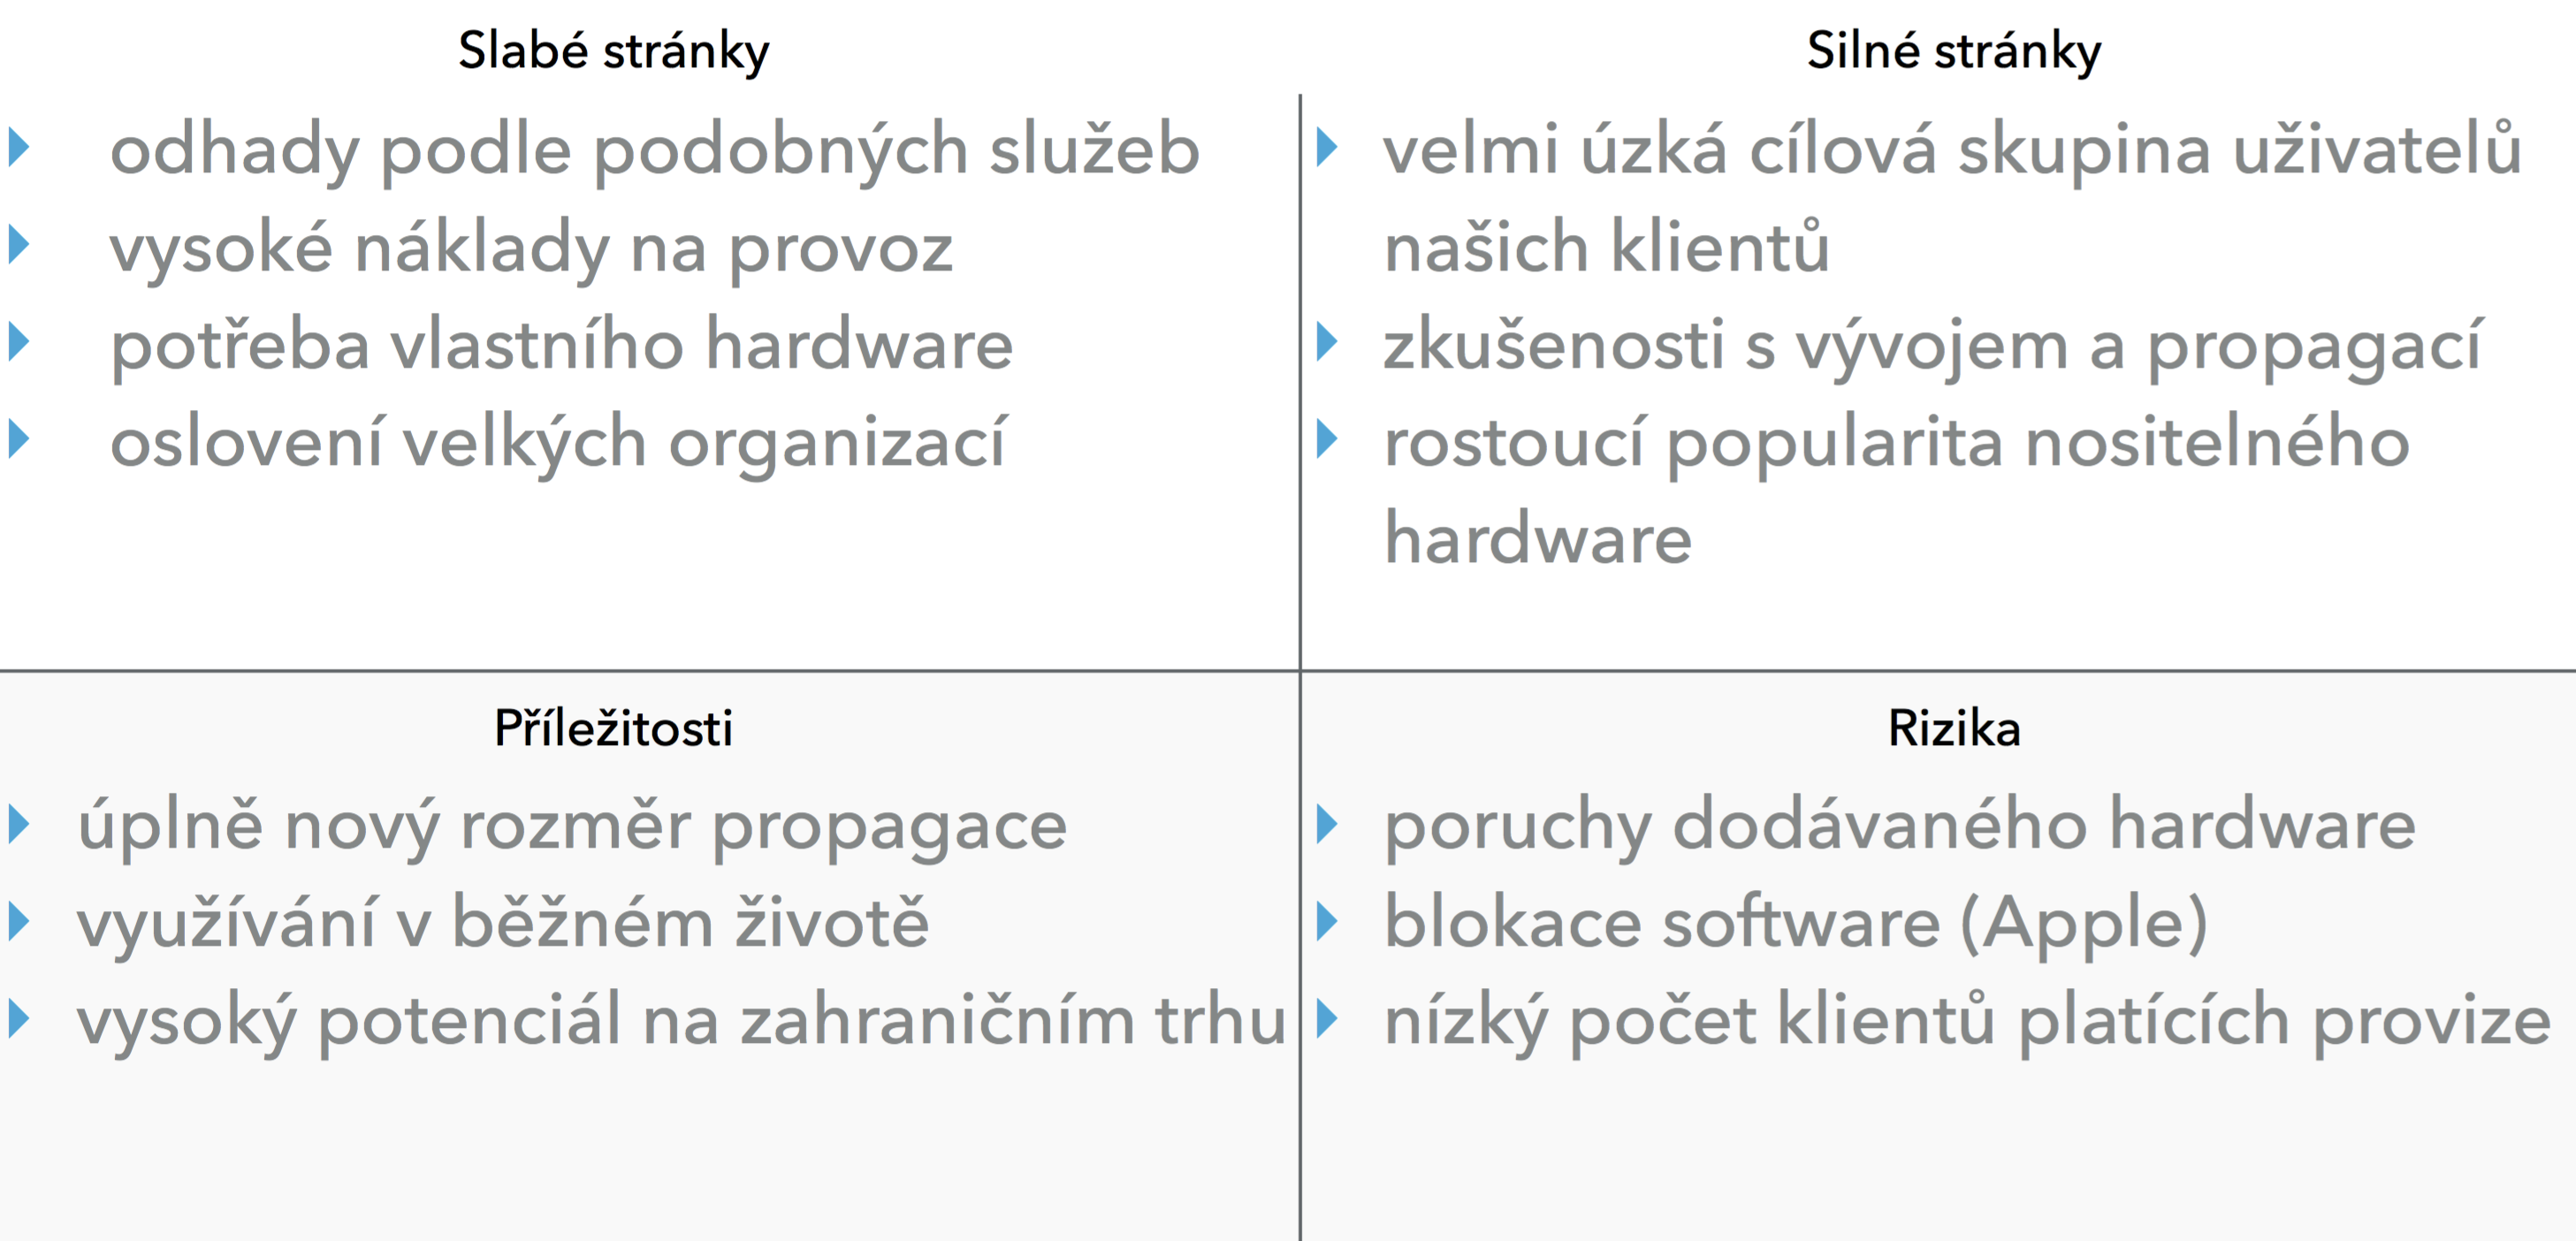
\includegraphics[width=\textwidth]{BI-EMP/project-plan/assets/swot}

\end{document}